\documentclass[12pt]{article}

\usepackage[utf8]{inputenc}
\usepackage[T2A]{fontenc}
\usepackage[english,russian]{babel}
\usepackage{amssymb}
\usepackage{graphicx}
\graphicspath{ {images/} }

\textwidth=431pt
\textheight=600pt
\hoffset=-30pt
\voffset=-30pt

\usepackage{graphicx}
\usepackage{amsmath}
\makeatletter
\renewcommand{\@oddhead}{%
\vbox{%
\hbox to \textwidth{\strut \textit{SABD, Problem set 2, Usvyatsov Mikhail} \hfill }
%\hbox to\textwidth{Лист\hfill Страница~\arabic{page}~из 2}
\hrule
\vspace{12pt}
}}
\renewcommand{\@oddfoot}{}
\makeatother


\begin{document}

%\tableofcontents

%\newpage

\begin{center}
\textbf{Problem set 2 \\
DUE: Mon. September 8, 2014 \\}
\end{center}

\newcounter{qcounter}

\bigskip
	
\textbf{Exercise 1}		
		
Compute the sample mean and standard deviation of growth and tradeshr.
\medskip
		
\textbf{Solution}

E(growth) = 1.9427
E(tradeshr) = 0.5647

$\sigma(growth) = 1.37736$
$\sigma(tradeshr) = 0.5378386$
\bigskip

\textbf{Exercise 2}
		
Estimate a regression of growth on tradeshr, using the “robust” option.

\begin{list}{\alph{qcounter})~}{\usecounter{qcounter}}
\item
What is the coefficient on tradeshr? Explain in words what it means. Is the numerical value of your estimate large or small in an economic (real-world) sense?
\item
Graph the data points and the estimated regression line.
\item
Is the slope coefficient statistically significantly different from zero at the 5\% significance level? Show how you reach this conclusion.
\item
Report the 95\% confidence interval for $\beta_1$ , the slope of the population regression line.
\item
What is the $R^2$ of this regression? What does this mean?
\item
Compute the correlation coefficient between growth and tradeshr, and compare its square to the $R^2$. How are the correlation coefficient and the $R^2$ related?
\item
What is the value of the root mean squared error of the regression? What does this mean?
\item
Based on your graph from (b), does the regression error appear to be homoskedastic or heteroskedastic?
\item
Run the regression again without the “robust” option. Compare the results to what you obtained with the “robust” option. What is different?
\item
You should see an outlier in the data set. Rerun the regression (with the “robust” option), dropping the outlier. Does dropping the outlier make a qualitative difference to your results? Explain.
\item
What is the outlying observation? Considering the economics of the relation you are investigating, in your judgment should that outlier be omitted from the regression? (You might need to do a bit of research about that outlier to answer this question properly.)
\end{list}
\medskip
		
\textbf{Solution}

\begin{list}{\alph{qcounter})~}{\usecounter{qcounter}}
\item
The slope coefficient on tradeshr is 2.2233374. It means that if tradeshr will be changed by one, growth will be changed in 2.2233374. I personally think that such value of slope parameter is large in a real-world sense.
\item
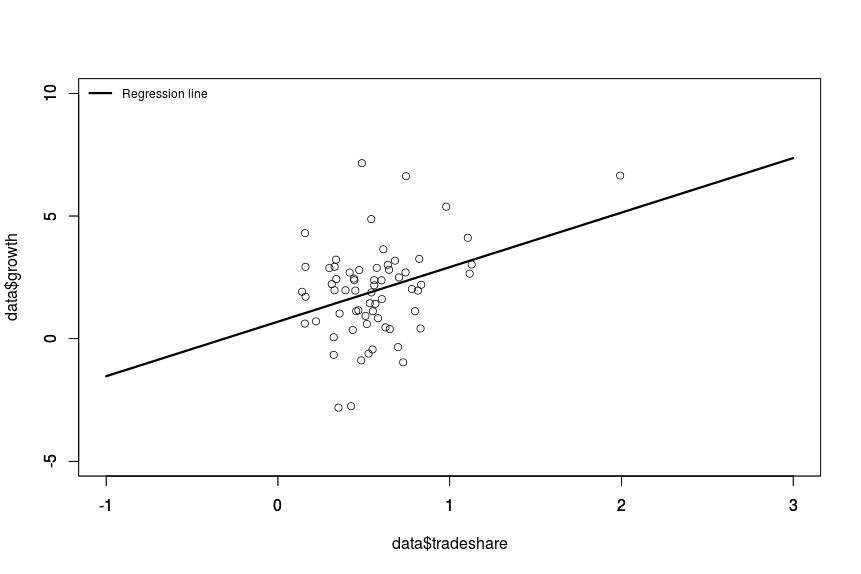
\includegraphics[width=1\textwidth]{Rplot.png}
\item
$t = \dfrac{\hat{\beta} - \beta_{1.0}}{SE(\hat{\beta})}$\\
$\beta_{1.0} = 0$\\
${SE(\hat{\beta})} = \sqrt{\hat{\sigma}^2_{\hat{\beta}}}$\\
$\hat{\sigma}^2_{\hat{\beta}} = \dfrac{1}{n} * \dfrac{\dfrac{1}{n-2} * \sum^{n}_{i = 1}(X_i - \overline{X})^2\hat{u}^2}{\left[\dfrac{1}{n} * \sum^{n}_{i = 1}(X_i-\overline{X})^2\right]^2}$\\
t = 3.2723 
t > 1.96, so we have to reject $H_0$
\item
$[\hat{\beta}_1 - 1.96*SE(\hat{\beta}_1),\hat{\beta}_1 + 1.96*SE(\hat{\beta}_1)] = [0.870643,3.576032]$
\item
$R^2 = \dfrac{ESS}{TSS} = \dfrac{\sum^{n}_{i=1}(\hat{Y}_i-\overline{Y})^2}{\sum^{n}_{i=1}(Y_i-\overline{Y})^2}=0.1149446$\\
It means that the regression on tradeshare predicts growth bad.
\item
$(corr(growth, tradeshare))^2 = 0.1236802$\\
As $R^2$
it shows that the value of tradeshare is not very much correlated with growth, however we cannot say that this values are not correlated.
\item
RMSE = $\sqrt{\dfrac{\sum^{n}_{i=1}\hat{u}^2_i}{n}}=1.7624$
\item
It seems to be heteroskedastic.
\item
According to the graphic of regressions, regression without robustness has a little bit different coefficients.
\item
According to the graphic of regressions, regression without the outlier has very different coefficients.
\item
Outlying observation is Malta. We have to omit the outlier because linear regression is sensitive for it.
\end{list}

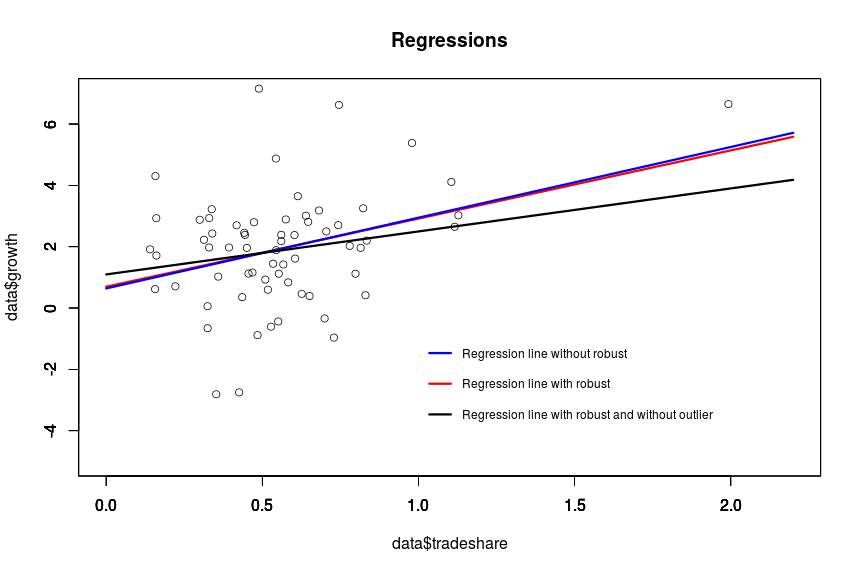
\includegraphics[width=1\textwidth]{Rplot1.png}

\textbf{Exercise 3}

Construct a new variable, lorgdp60, which equals one if the country’s GDP is in the
bottom quartile of GDP for 1960 and equals zero otherwise. Estimate a regression of
growth on lorgdp60, using the “robust” option.

\begin{list}{\alph{qcounter})~}{\usecounter{qcounter}}
\item
What is the coefficient on lorgdp60? Explain in words what this means. Is the
numerical value of your estimate large or small in an economic (real-world) sense?
\item
Test the hypothesis that the mean growth rate from 1960-1995 is the same for countries with lorgdp60 = 1 as it is for countries with lorgdp60 = 0, against the
alternative that they differ, at the 5\% significance level.
\item
Using the “summarize” command, compute the sample average of growth for
countries with lorgdp60 = 1 and then again for countries with lorgdp60 = 0; from
this compute the difference in mean GDP growth rates for the two groups and
construct the differences-of-means t-statistic testing the hypothesis that the mean
growth rates are the same.
\item
Reestimate the regression of growth on lorgdp60, without the “robust” option. How
does the t-statistic computed in (c) compare to the t-statistic on the slope coefficient in the regression of growth on lorgdp60 obtained with and without the “robust”
option? Explain.
\end{list}

\textbf{Solution}
\medskip

\begin{list}{\alph{qcounter})~}{\usecounter{qcounter}}
\item
$\hat{\beta}_1 = -1.640866$

It means that when lorgdp60 = 1 growth decreases by 1.64. In economic sense the value of the coefficient can be large.
\item
$t = \dfrac{\overline{Y}_m-\overline{Y}_n - d_0}{SE(\overline{Y}_m-\overline{Y}_n)}=2.284999$

So we have to reject the idea that the means are equal.
\item
Due to the fact that we didn't use stata this task is equal to previous one.
\item
The differences are in counting SE. When regression is robust we have to estimate the error $u_i$

$SE(\hat{\beta}_1) = \sqrt{\hat{\sigma}^2_{\hat{\beta}_1}}$

in robust case:\\
$\hat{\sigma}^2_{\hat{\beta}} = \dfrac{1}{n} * \dfrac{\dfrac{1}{n-2} * \sum^{n}_{i = 1}(X_i - \overline{X})^2\hat{u}^2}{\left[\dfrac{1}{n} * \sum^{n}_{i = 1}(X_i-\overline{X})^2\right]^2}$

in not robust case:\\
$\widetilde{\sigma}^2_{\hat{\beta}} = \dfrac{s^2_{\hat{u}}}{\sum^{n}_{i = 1}(X_i-\overline{X})^2}$
\end{list}

\textbf{Exercise 4}
\bigskip

Table 2 presents the results of three regressions, one in each column. Estimate the indicated regressions and fill in the values (you may either handwrite or type the entries in, at you convenience; if you choose to type up the table, an electronic copy of Table 2 in .doc format is available on the course Web site). For example, to fill in column (1), estimate the regression with growth as the dependent variable and tradeshr and school60 as the independent variables, using the “robust” option, and fill in the estimated coefficients and standard errors; also compute and fill in the value of the F-statistic and p-value testing the hypothesis that the coefficients on tradeshr and school60 are both zero. The adjusted $R^2$ can be computed by rerunning this regression without the “robust” option. Note: the regressions in Table 2 all exclude the observation on Malta.\\

\textbf{Solution}
\medskip

\begin{tabular}{| l | c | c |r |}
  \hline
  {\bf Regressor} & {\bf (1)} & {\bf (2)} & {\bf (3)}\\ \hline
  tradeshare & (1.5412032) & (1.3686513435) & (0.8505190649)\\ \hline
  school60 & (0.2105808) & (0.4730324670) & (0.4478457993)\\ \hline
  capstock60 & - & (-0.0003034976) & (-0.0003690296)\\ \hline
  revc & - & - & (-2.7211122223)\\ \hline
  civil & - & - & ( 0.3973022112)\\ \hline
  Intercept & 0.0972978 & 0.1509167230 & 1.0709842944 \\ \hline
  
   \multicolumn{4}{|p{15cm}|}{\bf F-statistics testing the hypothesis that the population coefficients on the indicated regressors are all zero:}  \\ \hline
  tradeshare, school60 & (4.152) & (5.5003) & (4.6298)\\ \hline
  tradeshare, school60, capstock60 & - & (3.9728) & ( 3.0852)\\ \hline
  revc, civil & - & - & (5.1212)\\ \hline
  \multicolumn{4}{|l|}{\bf Regression summary statistics}  \\ \hline
  $\overline{R^2}$  & 0.1331  & 0.2078   &0.23  \\ \hline
  $R^2$ & 0.1606 & 0.2455 &0.2911 \\ \hline
  Regression RMSE & 1.65775 & 1.572138 & 1.534965\\ \hline
  n & 64  & 64  & 64 \\ \hline
\end{tabular}

\textbf{Exercise 5}
\bigskip

Use Table 2 to answer the following questions.
\newcounter{acounter}
\begin{list}{\alph{acounter}) ~}{\usecounter{acounter}}
\item Write the regression in column (1) in “equation form,” with the standard error below the respective regression coefficient.
\item Explain in words what the coefficient on school60 means in regression (1).
\item Using regression (1), test the hypothesis that the coefficient on tradeshr is zero, against the alternative that it is nonzero, at the 5\% significance level. In everyday words (not statistical terms), what precisely is the hypothesis that you are testing?
\item Does the coefficient on tradeshr differ in regressions (1), (2), and (3) in a substantively important way, that is, is the difference between the three estimates large in a real-world sense?
\item Economic theory predicts that tradeshr, school60, and capstock60 all are determinants of economic growth. Use regression (2) to test the hypothesis (at the 5\% significance level) that the coefficients on these three economic variables are all zero, against the alternative that at least one coefficient is nonzero.
\item In regression (3), is the coefficient on revc statistically significant at the 5\% significance level? Is the coefficient on civil statistically significant at the 5\% significance level? 
\item Use the heteroskedasticity-robust F-statistic to test the hypothesis (at the 1\% significance level) that the coefficients on the political variables (revc and civil) in regression (3) are both zero, against the alternative that one or the other or both are nonzero. Discuss in light of your answer to part (f).
\item The neoclassical theory of human capital in economics suggests that countries with more human capital – that is, a better educated work force – will have a higher rate of productivity and therefore have a higher growth rate. Is this prediction borne out in the regression results? Explain.
\end{list}

\textbf{Solution}
\medskip
\newcounter{bcounter}
\begin{list}{\alph{bcounter}) ~}{\usecounter{bcounter}}
\item 
\begin{tabular}{ccccccc}
$0.0972978$ & $+$ & $1.5412032$ & $tradeshare$ & $+$ & $1.5412032$ & $school60$\\
$\left(0.71071231\right)$ & \ & \ & $\left(0.91985029\right)$ & \ & \ & $\left(0.07660823\right)$\\
\end{tabular}

\item 
The school60 means that it has increased/decreased by one the growth increased by 0.07660823.

\item $t = \dfrac{\hat{\beta_{1}}-\beta_{1}}{SE(\hat{\beta_{1}})} = \dfrac{1.5412032}{0.91985029}=1.667301$

$\left|t\right|<1.96$ -the hypothesis is accepted in 5\% significance level.

\item decrease importance of regressors during increasing of number of regressors

\item Lets calculate F-test for this hypothesis from R

$regr<-lmRob(newData\$growth~newData\$tradeshare+newData\$yearsschool+newData\$rgdp60)$
$anova(regr, lmRob(newData\$growth~1))$

The F-test is:

$F=3.9728$

$F>2.6$ - hence, hypothesis is rejected in 5\% significance level.

\item Lets calculate the standards error for equation

\begin{tabular}{ccccccccccccc}
$1.071$ & $+$ & \shortstack{$0.851$ \\ $tradeshare$} & $+$ & \shortstack{$0.448$ \\ $yearsschool$} & $-$ & \shortstack{$0.0004$ \\ $rgdp60$} & $-$ & \shortstack{$2.721$ \\ $rev\_coups$} & $+$ & \shortstack{$0.397$ \\ $assasinations$}\\
$\left(0.6664\right)$ & \ & $\left(0.8171\right)$ \ & \ & $\left(0.1218\right)$ & \ & $\left(0.0001\right)$ & \ & $\left(0.952\right)$ & \ & $\left(0.4153\right)$
\end{tabular}

And calculate t-test

For coefficient on revc

$t = \dfrac{\hat{\beta_{revc}}-\beta_{revc}}{SE(\hat{\beta_{revc}})} = \dfrac{2.721}{0.952}=2.858193$

$\left|t\right|>1.96$ -the hypothesis is rejected in 5\% significance level.

For coefficient on assasinations
$t = \dfrac{\hat{\beta_{as}}-\beta_{as}}{SE(\hat{\beta_{as}})} = \dfrac{0.397}{0.4153}=0.9559355$

$\left|t\right|<1.96$ -the hypothesis is accepted in 5\% significance level.

\item Lets calculate robust F-test in R

$anova(lmRob(newData\$growth~newData\$tradeshare+newData\$yearsschool+newData\$rgdp60+newData\$rev_coups+newData\$assasinations), lmRob(newData\$growth~newData\$tradeshare+newData\$yearsschool+newData\$rgdp60))$

$F = 5.1212$

$\left|F\right|>4.61$ - the hypothesis is rejected in 1\% significance level. 
\item
According to the coefficients, yearsschool doesn't have the biggest influence on growth. So the theory fails.
\end{list}
\end{document}